
% %map showing core locations
% \begin{figure}
% \centering
% 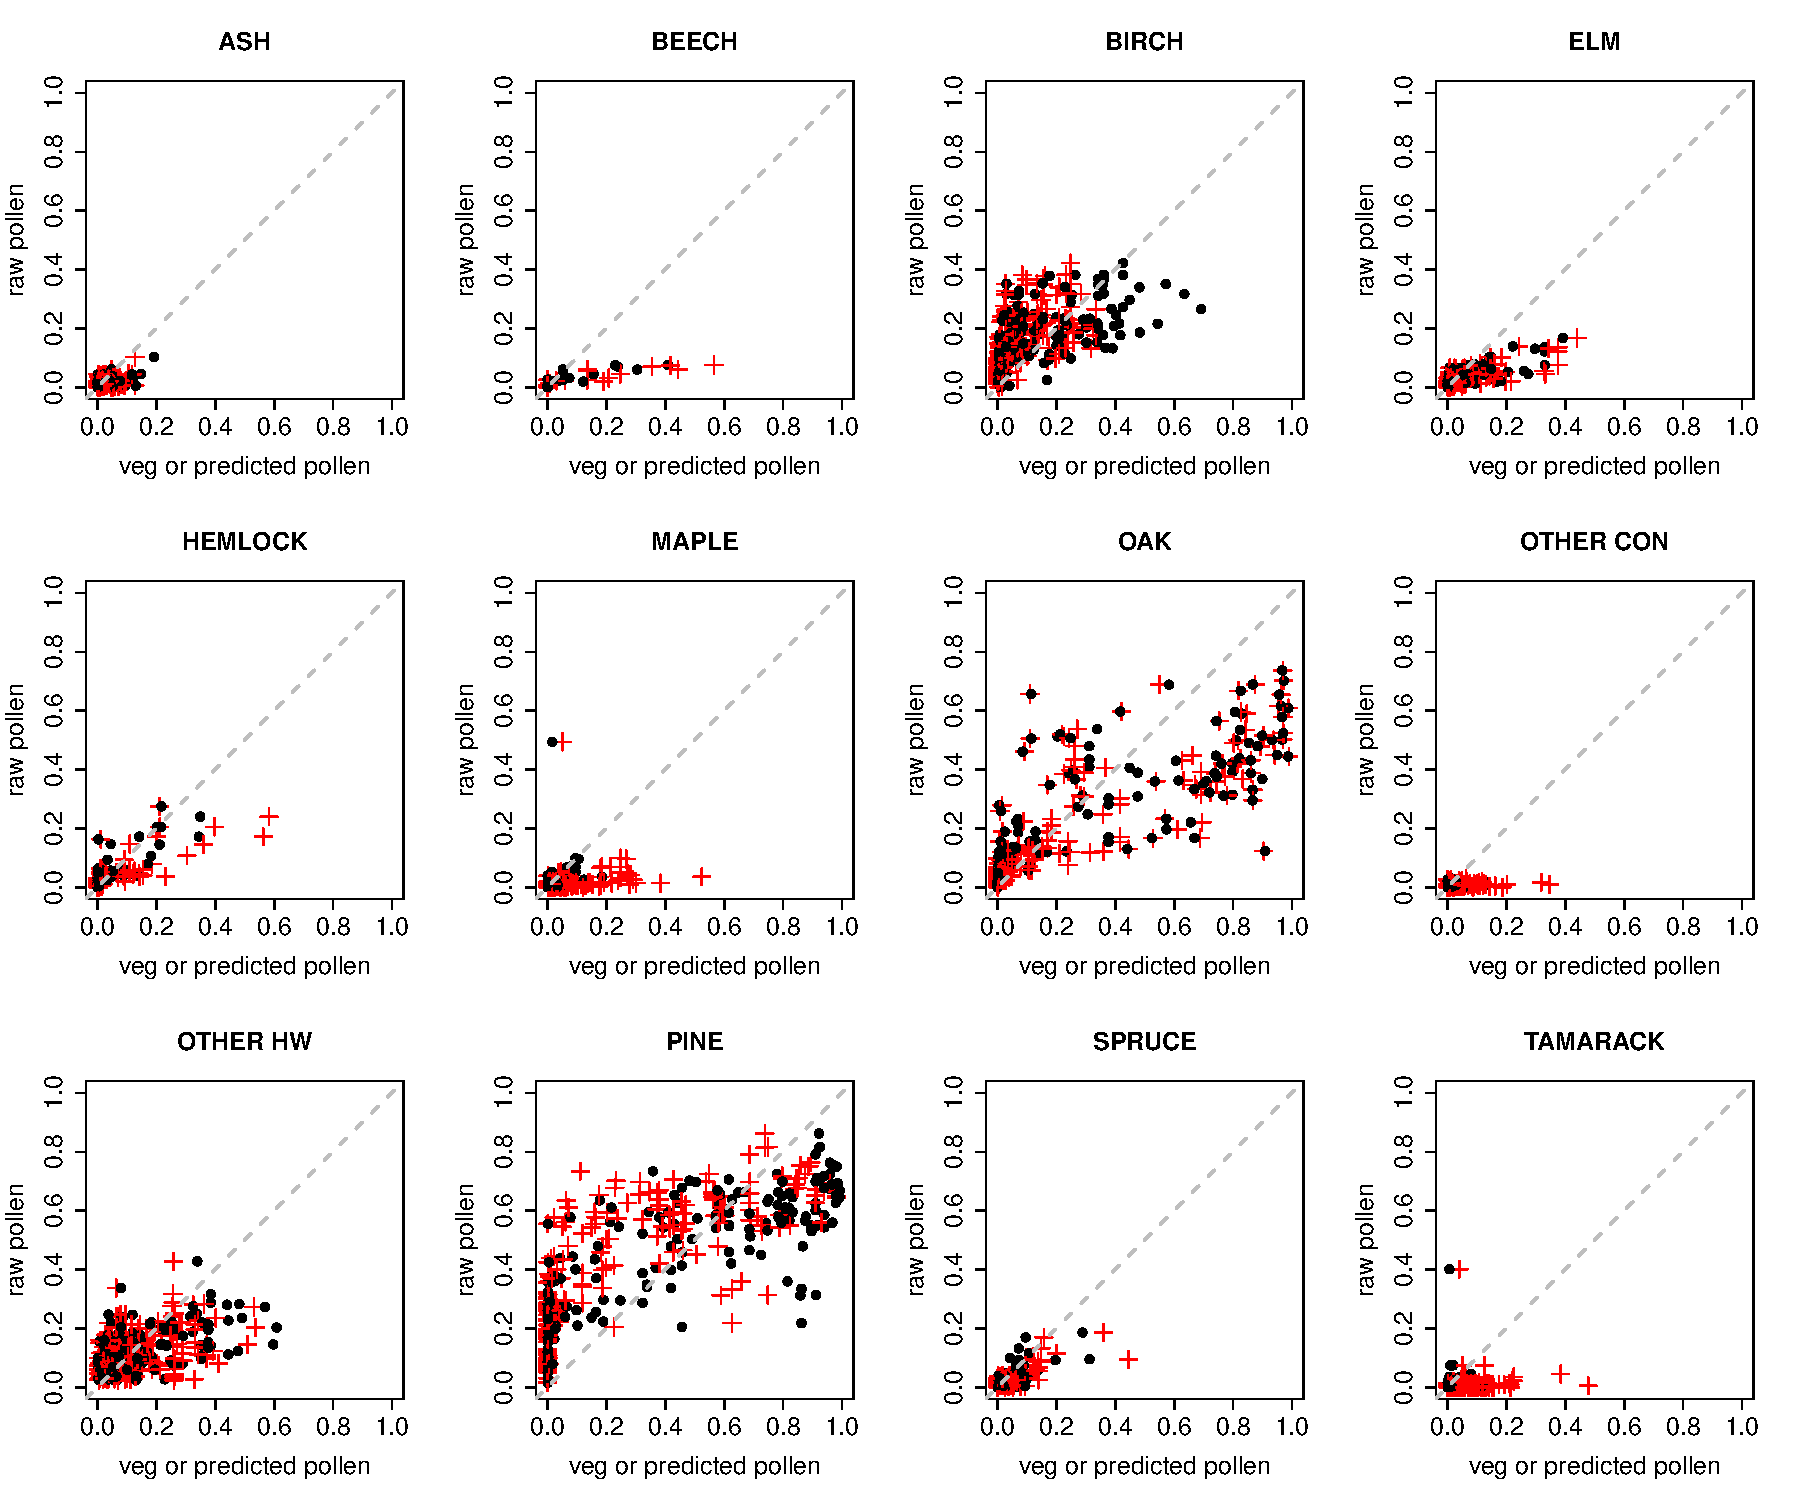
\includegraphics[width=7in]{figures/pollen_focal_scaled.pdf}
% \caption{}
% \label{fig:focal_scaled}
% \end{figure}

%map showing core locations
\begin{figure}
\centering
\begin{tabular}{c}
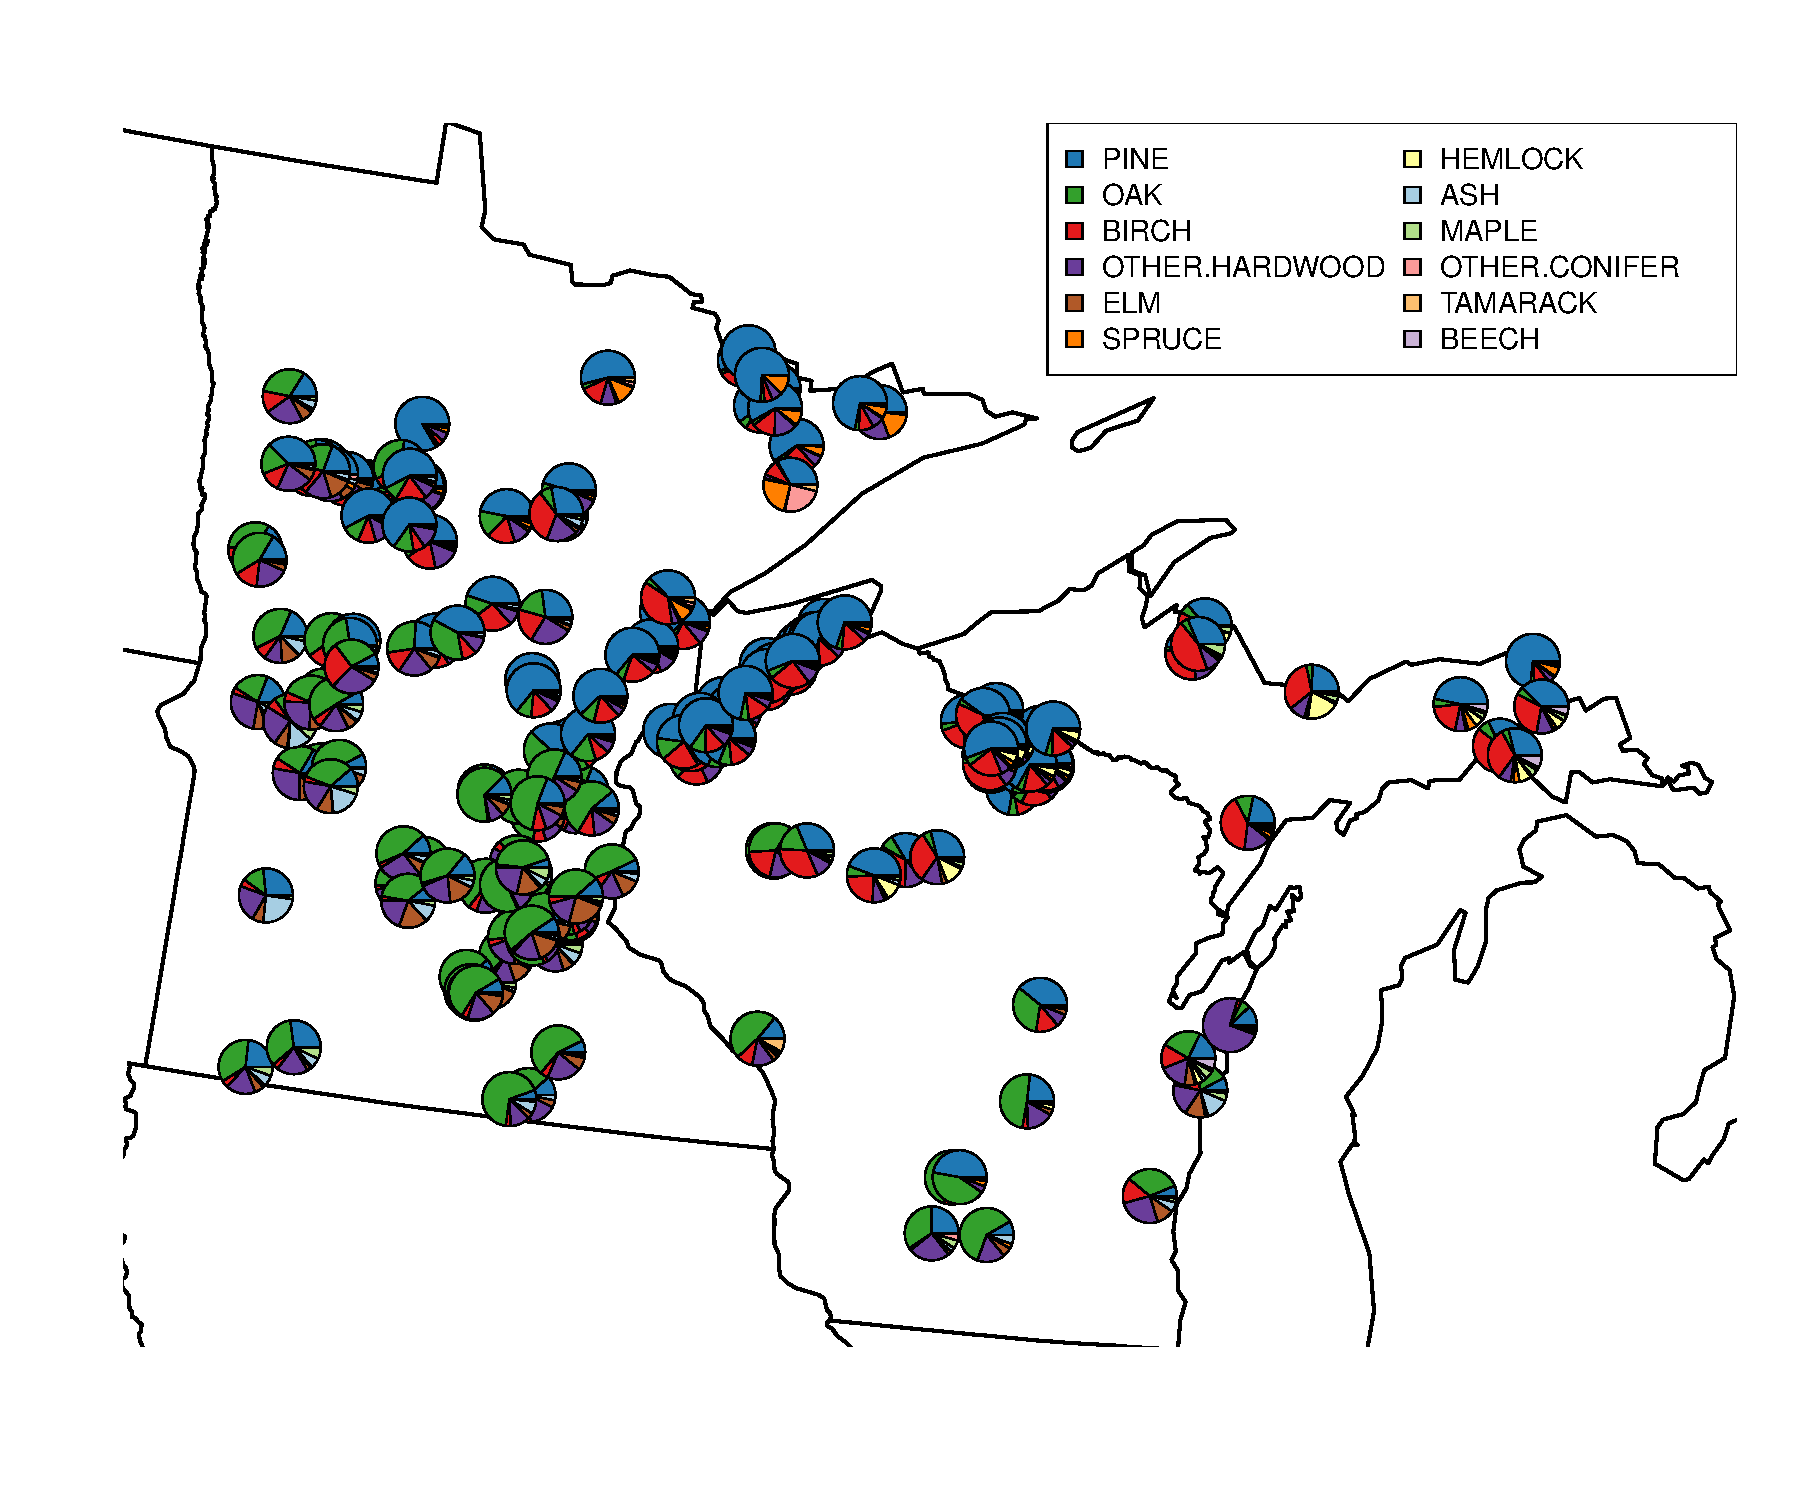
\includegraphics[width=5in]{figures/pie_plot_pollen_UMW_v01.pdf} \\
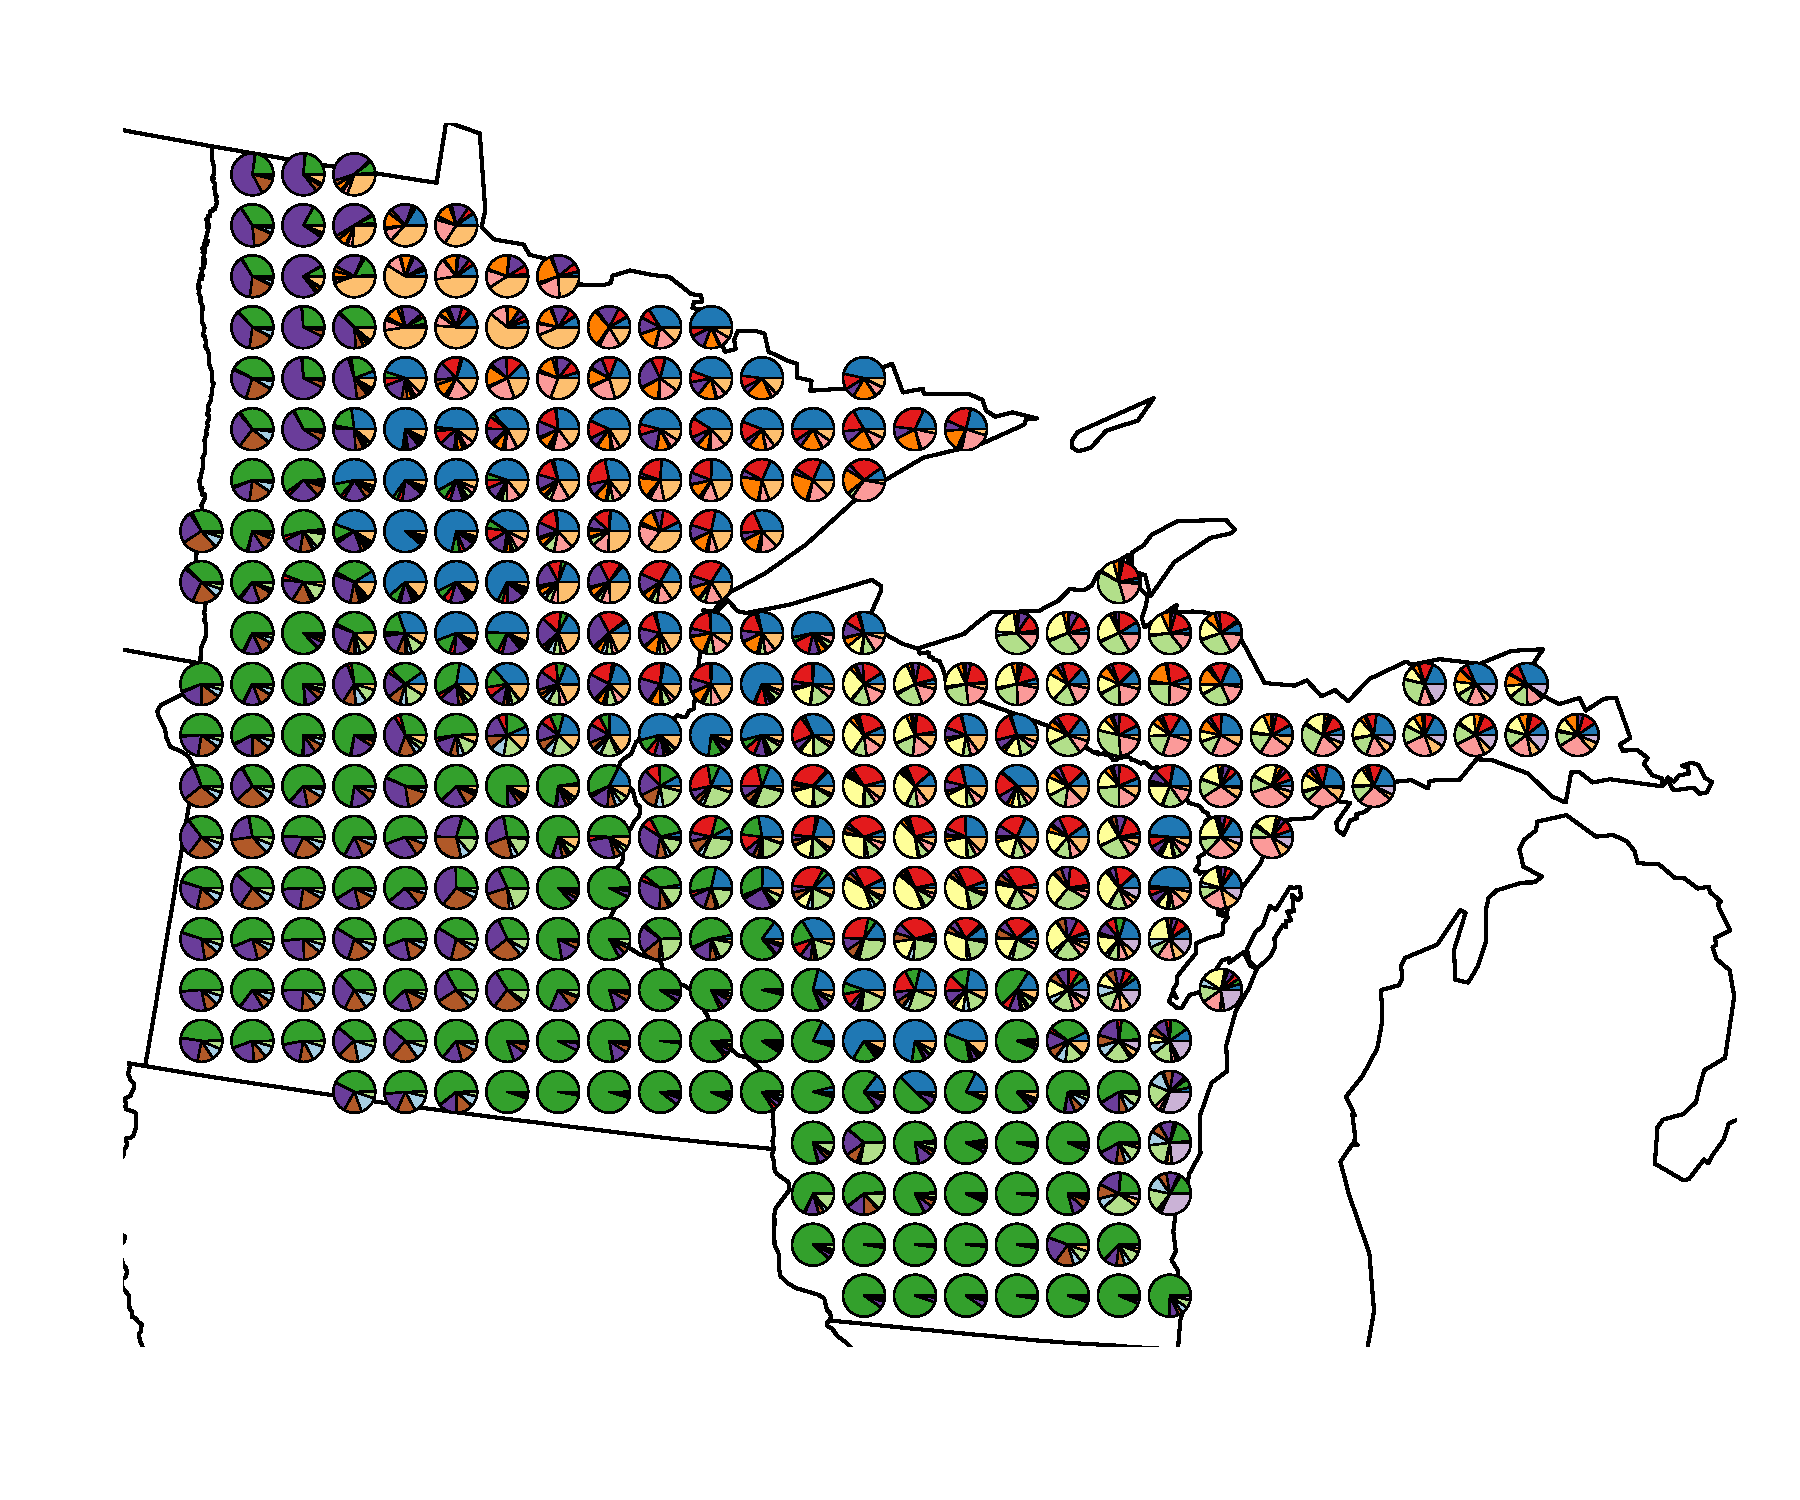
\includegraphics[width=5in]{figures/pie_plot_pls_UMW_v01.pdf}
\end{tabular}
\caption{}
\label{fig:pie}
\end{figure}

%pollen raw versus scaled focal
\begin{figure}
\centering
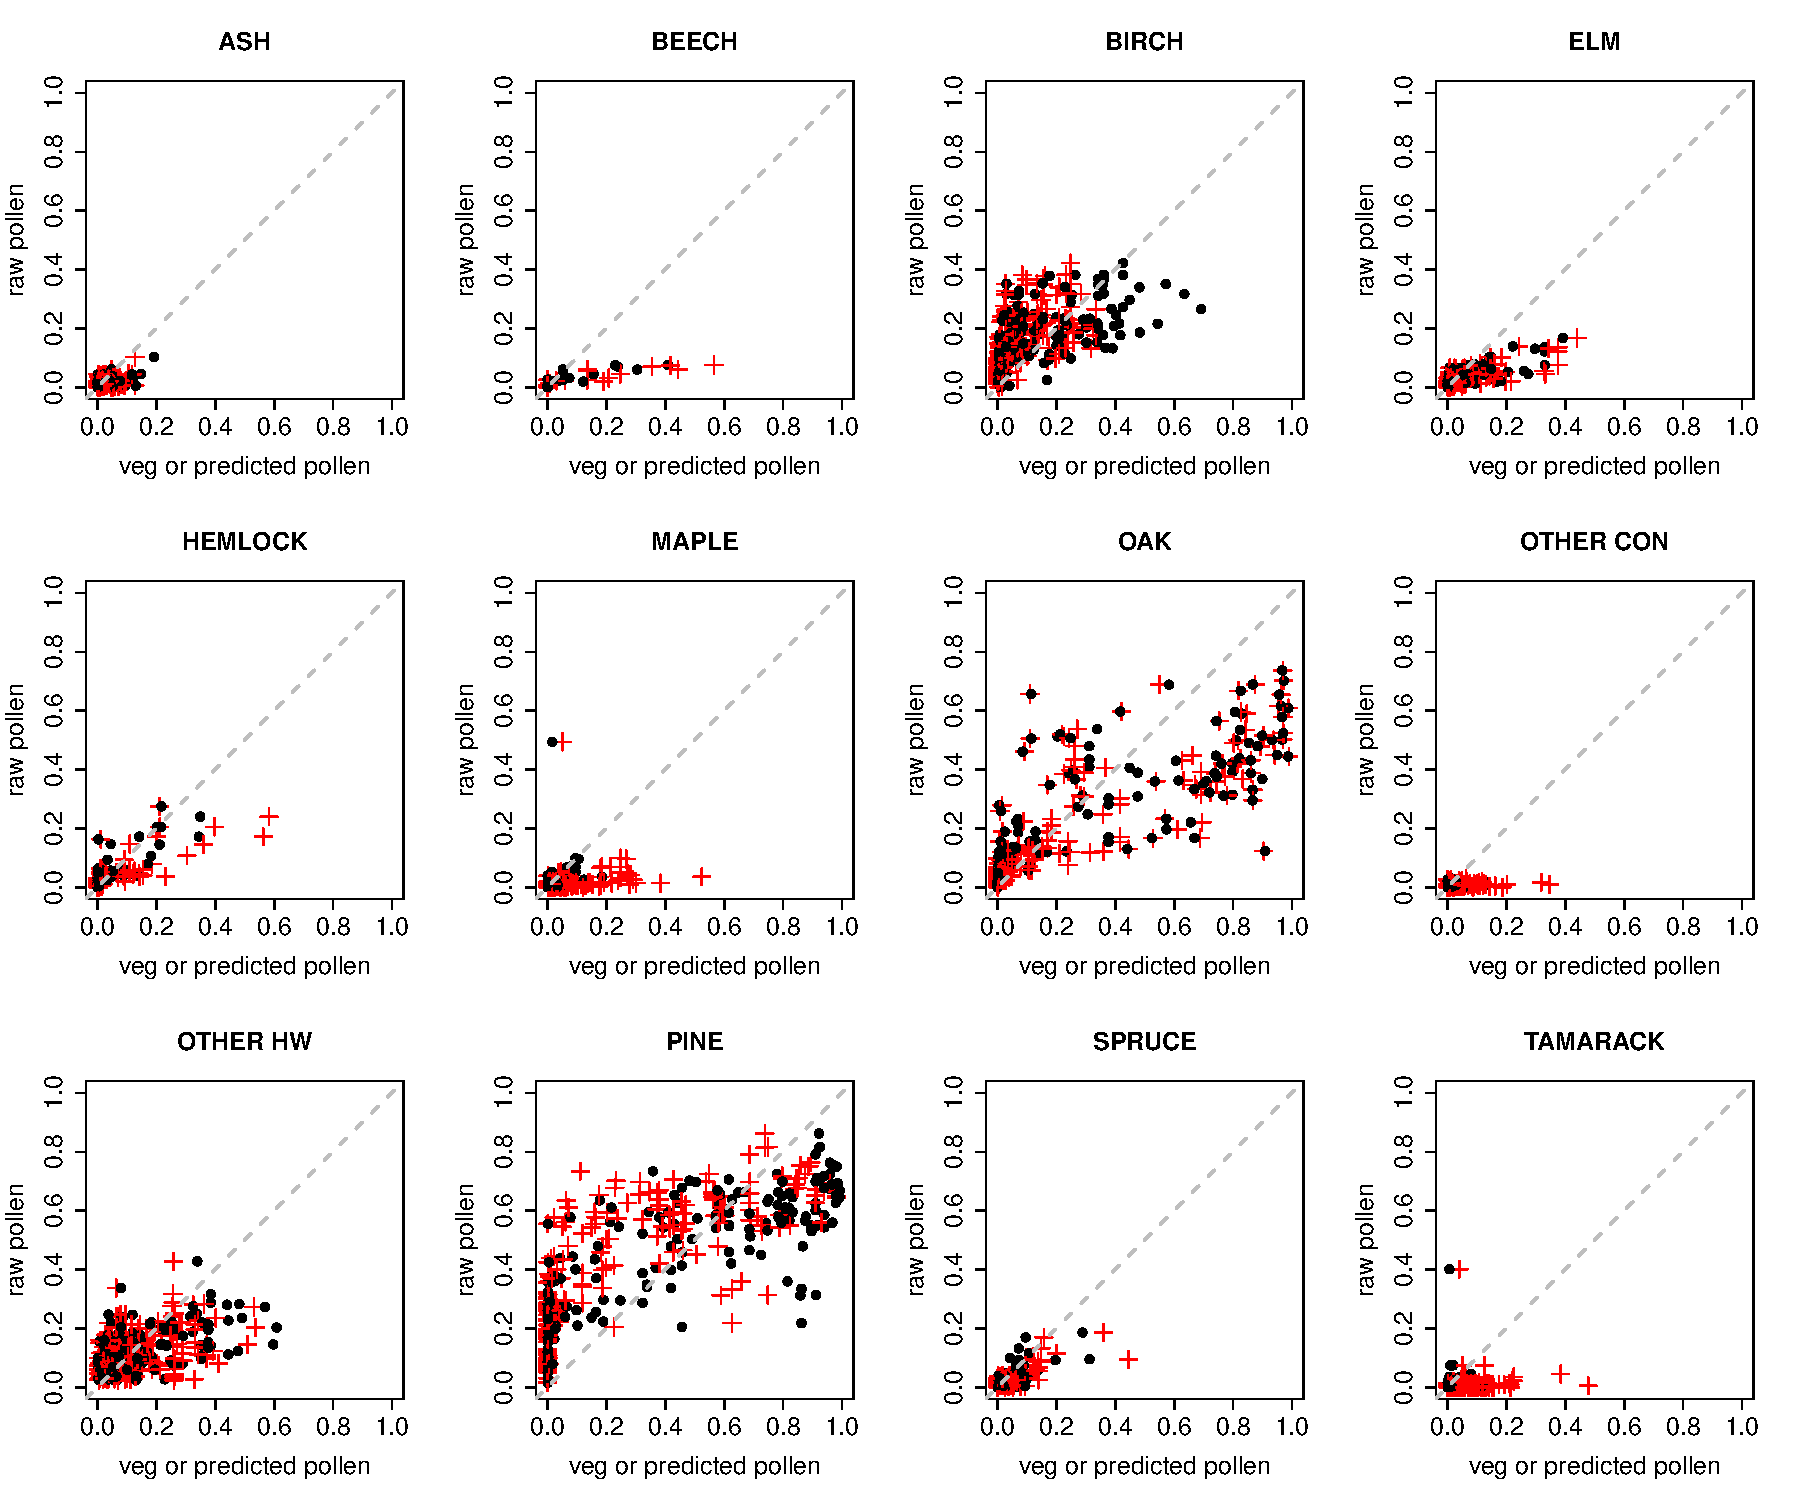
\includegraphics[width=7in]{figures/pollen_focal_scaled.pdf}
\caption{}
\label{fig:focal_scaled}
\end{figure}

%pollen raw versus predicted
\begin{figure}
\centering
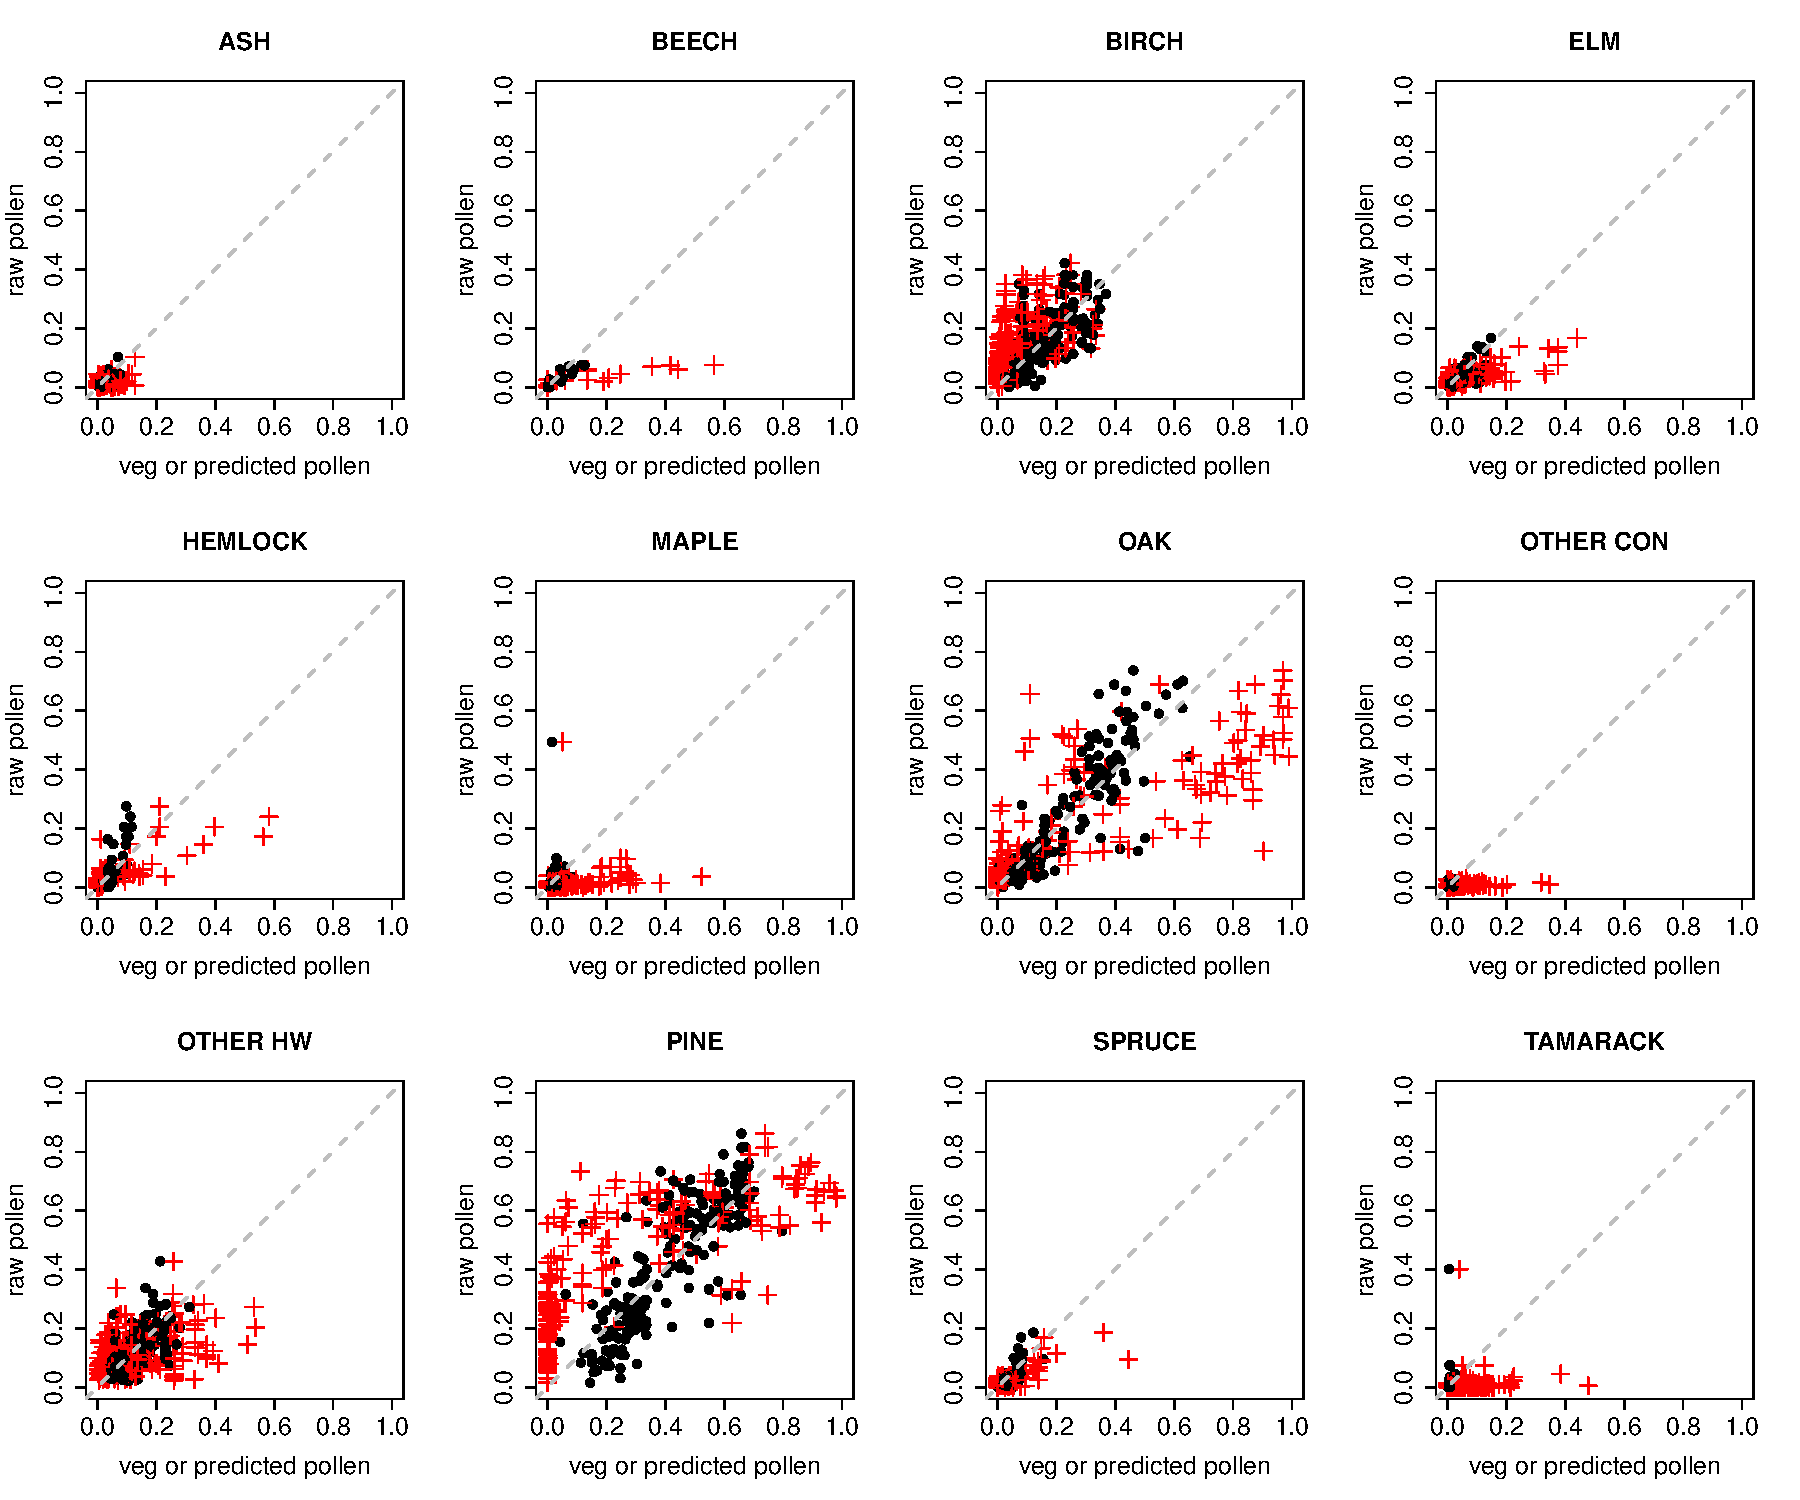
\includegraphics[width=7in]{figures/pollen_preds.pdf}
\caption{}
\label{fig:preds}
\end{figure}

%pollen raw versus predicted
\begin{figure}
\centering
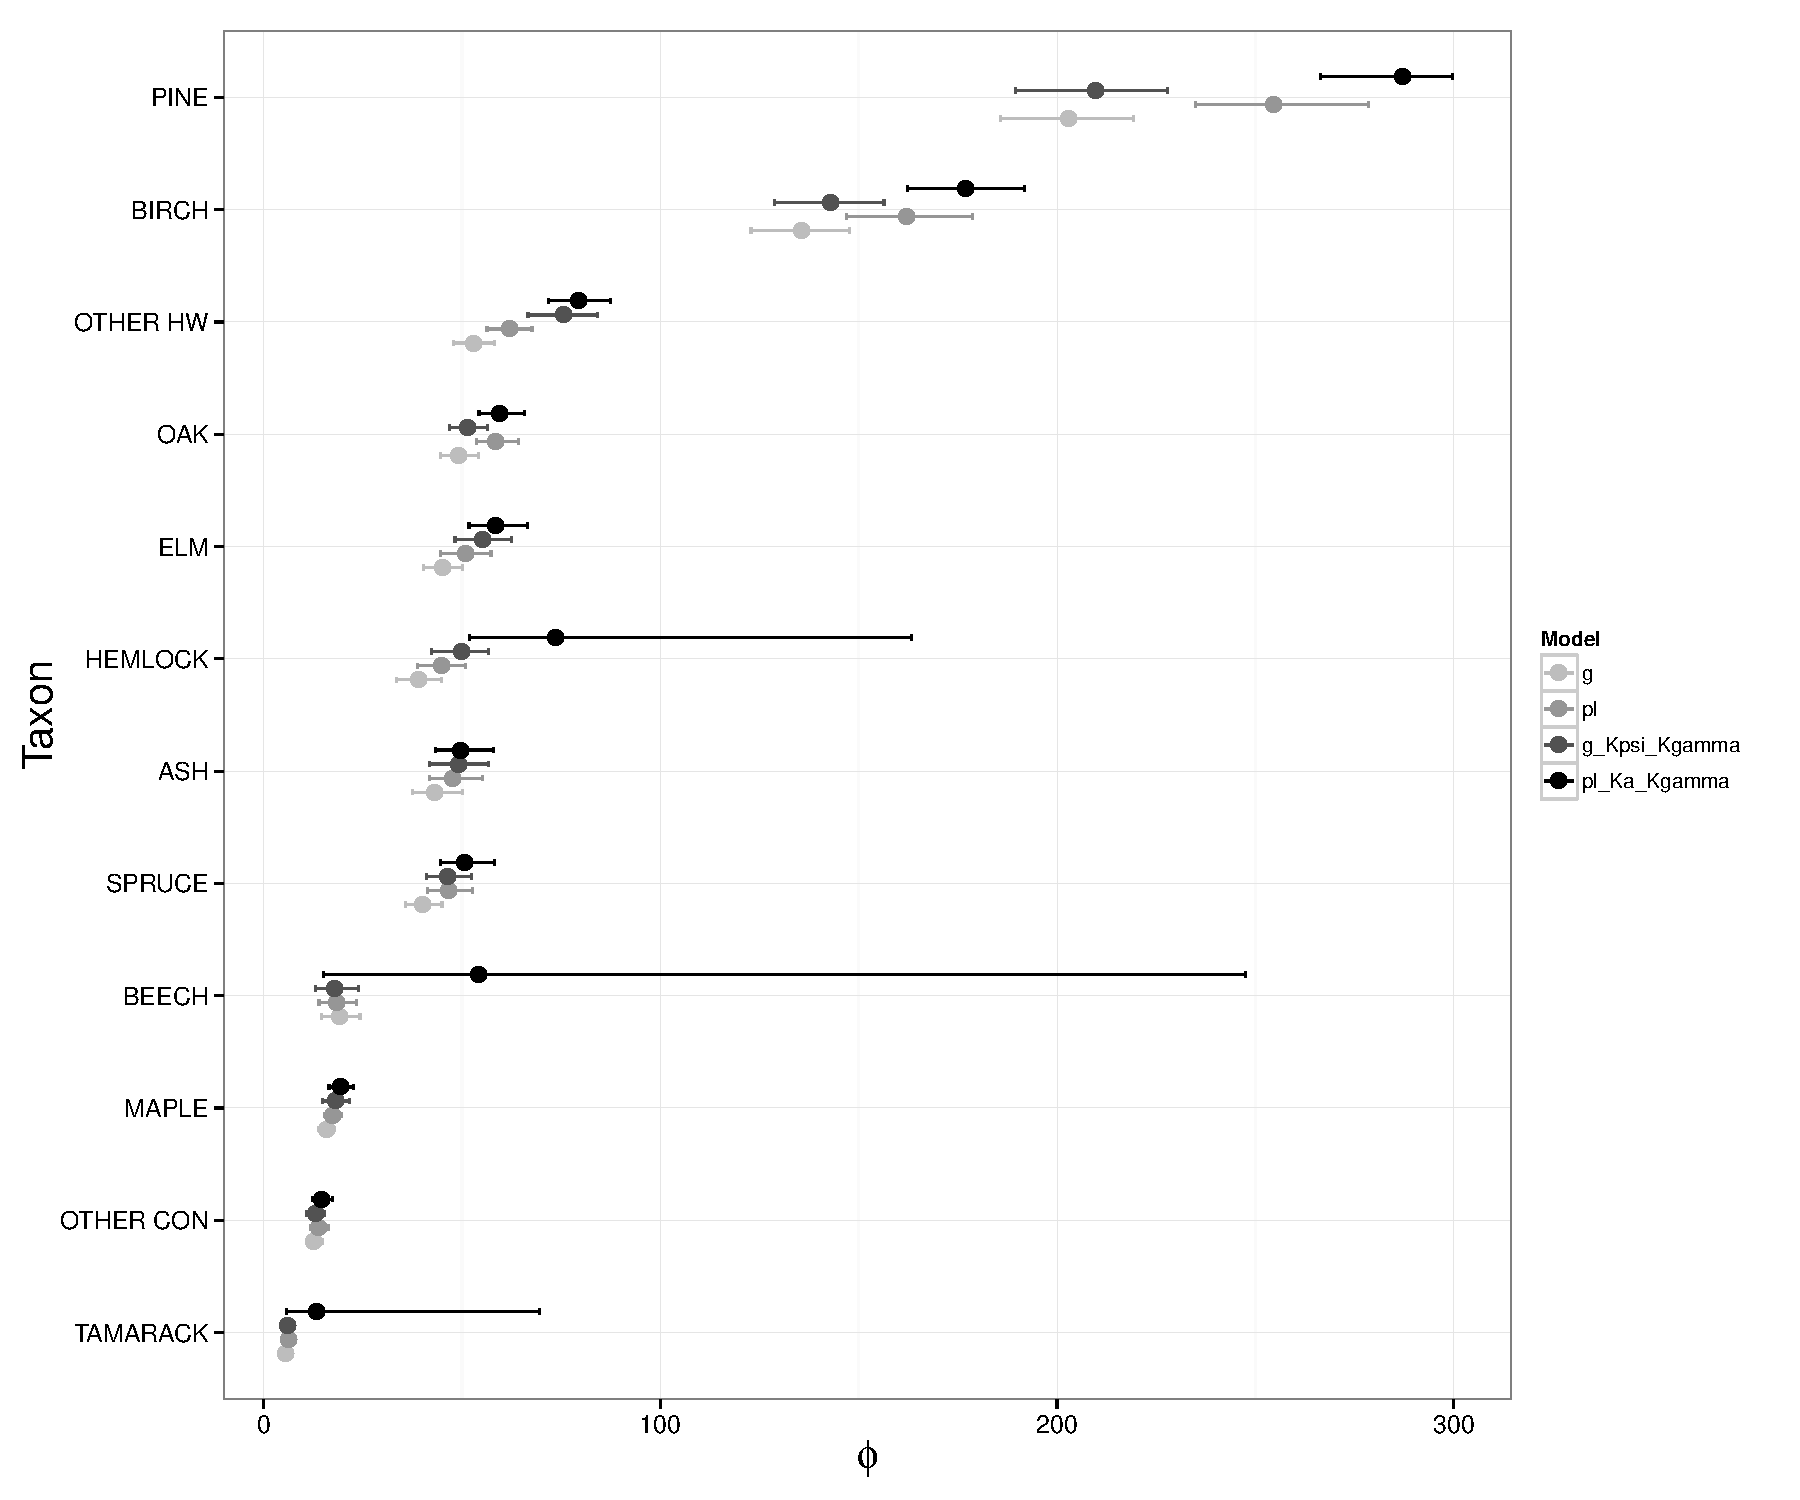
\includegraphics[width=7in]{figures/phi.pdf}
\caption{}
\label{fig:phi}
\end{figure}

%proportion pollen deposited versus radius
\begin{figure}
\centering
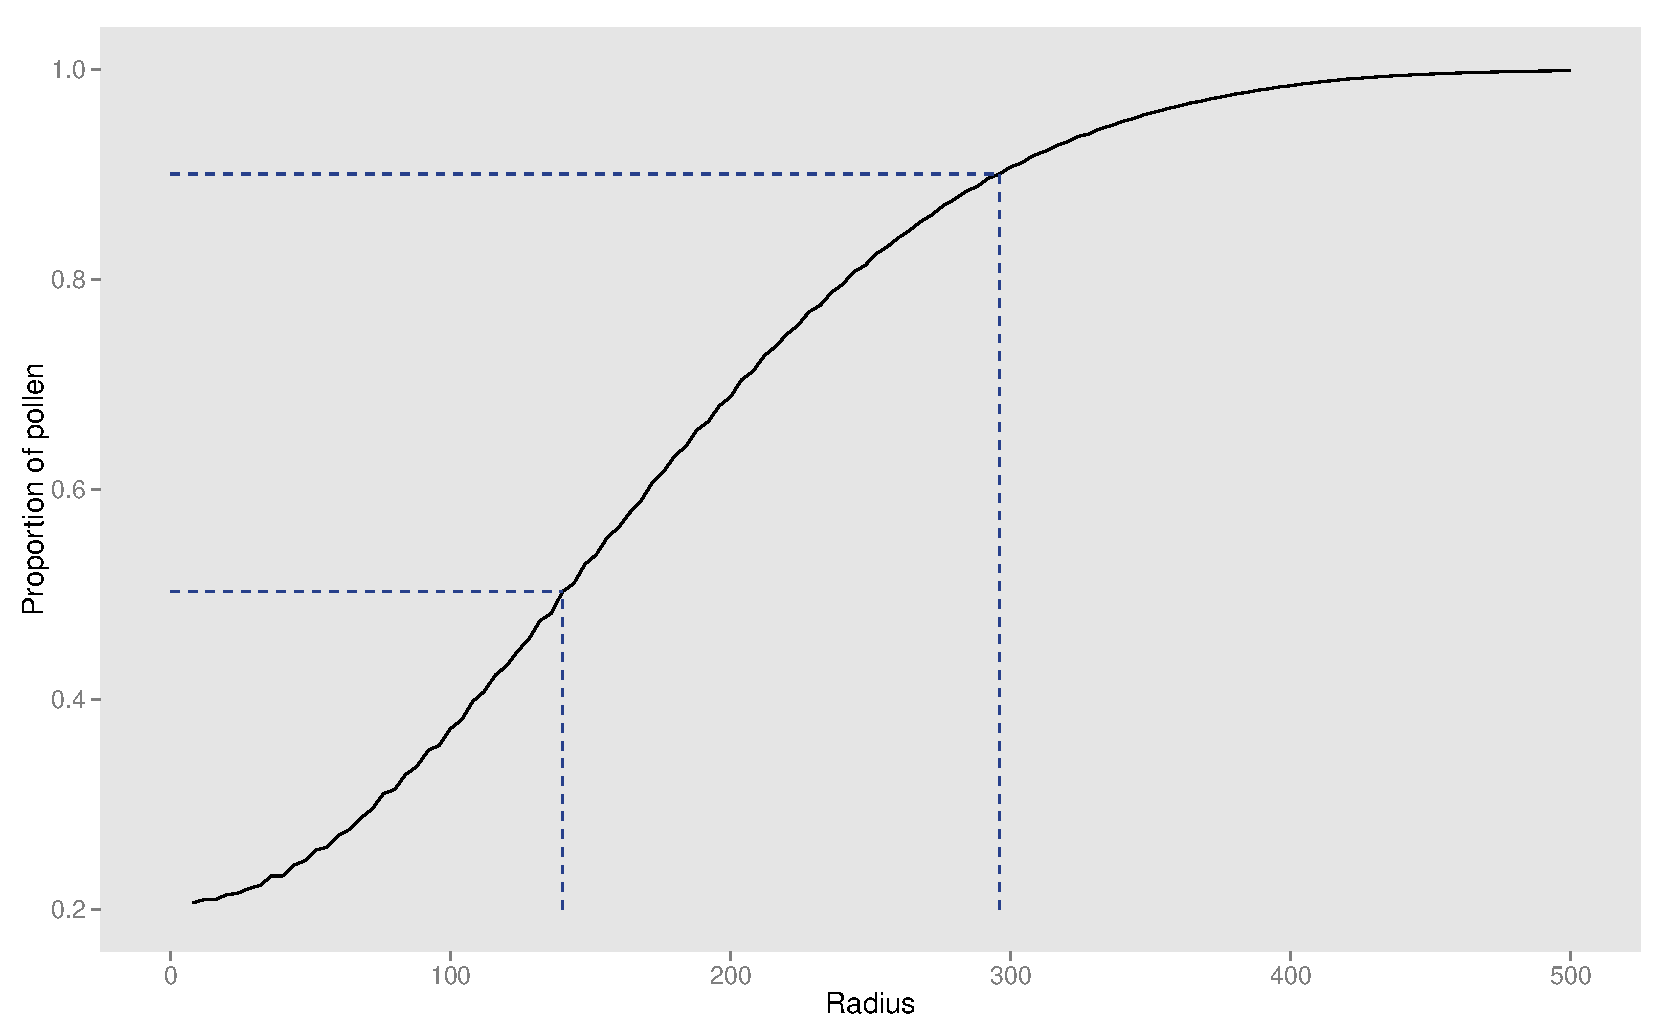
\includegraphics[width=7in]{figures/dispersal_vs_distance.pdf}
\caption{}
\label{fig:dvd}
\end{figure}

%proportion pollen deposited versus radius
\begin{figure}
\centering
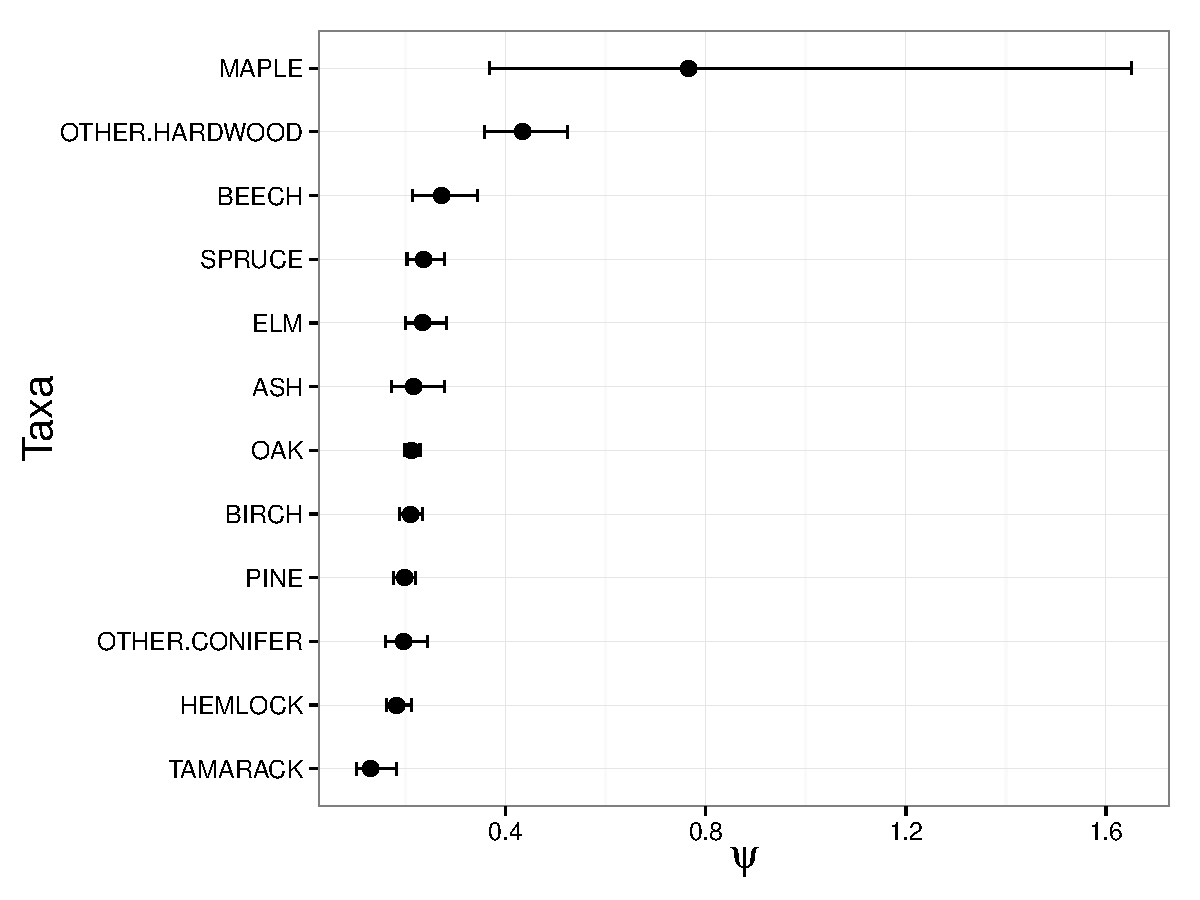
\includegraphics[width=7in]{figures/psi_vary_psi.pdf}
\caption{}
\label{fig:psi_vary_psi}
\end{figure}

%proportion pollen deposited versus radius
\begin{figure}
\centering
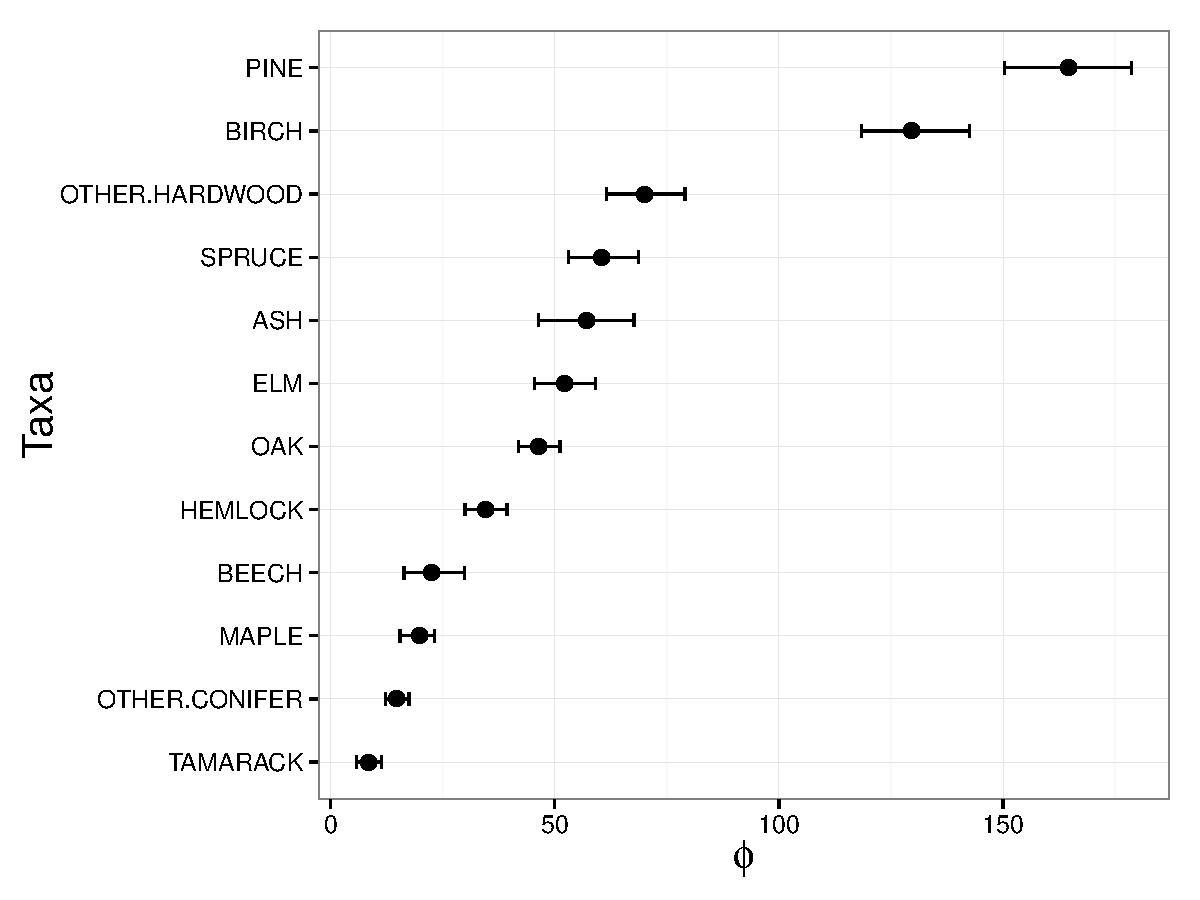
\includegraphics[width=7in]{figures/phi_vary_psi.pdf}
\caption{}
\label{fig:phi_vary_psi}
\end{figure}

